% Options for packages loaded elsewhere
\PassOptionsToPackage{unicode}{hyperref}
\PassOptionsToPackage{hyphens}{url}
%
\documentclass[
]{article}
\usepackage{lmodern}
\usepackage{amsmath}
\usepackage{ifxetex,ifluatex}
\ifnum 0\ifxetex 1\fi\ifluatex 1\fi=0 % if pdftex
  \usepackage[T1]{fontenc}
  \usepackage[utf8]{inputenc}
  \usepackage{textcomp} % provide euro and other symbols
  \usepackage{amssymb}
\else % if luatex or xetex
  \usepackage{unicode-math}
  \defaultfontfeatures{Scale=MatchLowercase}
  \defaultfontfeatures[\rmfamily]{Ligatures=TeX,Scale=1}
\fi
% Use upquote if available, for straight quotes in verbatim environments
\IfFileExists{upquote.sty}{\usepackage{upquote}}{}
\IfFileExists{microtype.sty}{% use microtype if available
  \usepackage[]{microtype}
  \UseMicrotypeSet[protrusion]{basicmath} % disable protrusion for tt fonts
}{}
\makeatletter
\@ifundefined{KOMAClassName}{% if non-KOMA class
  \IfFileExists{parskip.sty}{%
    \usepackage{parskip}
  }{% else
    \setlength{\parindent}{0pt}
    \setlength{\parskip}{6pt plus 2pt minus 1pt}}
}{% if KOMA class
  \KOMAoptions{parskip=half}}
\makeatother
\usepackage{xcolor}
\IfFileExists{xurl.sty}{\usepackage{xurl}}{} % add URL line breaks if available
\IfFileExists{bookmark.sty}{\usepackage{bookmark}}{\usepackage{hyperref}}
\hypersetup{
  pdftitle={512 Project},
  pdfauthor={Nolan Walker},
  hidelinks,
  pdfcreator={LaTeX via pandoc}}
\urlstyle{same} % disable monospaced font for URLs
\usepackage[margin=1in]{geometry}
\usepackage{color}
\usepackage{fancyvrb}
\newcommand{\VerbBar}{|}
\newcommand{\VERB}{\Verb[commandchars=\\\{\}]}
\DefineVerbatimEnvironment{Highlighting}{Verbatim}{commandchars=\\\{\}}
% Add ',fontsize=\small' for more characters per line
\usepackage{framed}
\definecolor{shadecolor}{RGB}{248,248,248}
\newenvironment{Shaded}{\begin{snugshade}}{\end{snugshade}}
\newcommand{\AlertTok}[1]{\textcolor[rgb]{0.94,0.16,0.16}{#1}}
\newcommand{\AnnotationTok}[1]{\textcolor[rgb]{0.56,0.35,0.01}{\textbf{\textit{#1}}}}
\newcommand{\AttributeTok}[1]{\textcolor[rgb]{0.77,0.63,0.00}{#1}}
\newcommand{\BaseNTok}[1]{\textcolor[rgb]{0.00,0.00,0.81}{#1}}
\newcommand{\BuiltInTok}[1]{#1}
\newcommand{\CharTok}[1]{\textcolor[rgb]{0.31,0.60,0.02}{#1}}
\newcommand{\CommentTok}[1]{\textcolor[rgb]{0.56,0.35,0.01}{\textit{#1}}}
\newcommand{\CommentVarTok}[1]{\textcolor[rgb]{0.56,0.35,0.01}{\textbf{\textit{#1}}}}
\newcommand{\ConstantTok}[1]{\textcolor[rgb]{0.00,0.00,0.00}{#1}}
\newcommand{\ControlFlowTok}[1]{\textcolor[rgb]{0.13,0.29,0.53}{\textbf{#1}}}
\newcommand{\DataTypeTok}[1]{\textcolor[rgb]{0.13,0.29,0.53}{#1}}
\newcommand{\DecValTok}[1]{\textcolor[rgb]{0.00,0.00,0.81}{#1}}
\newcommand{\DocumentationTok}[1]{\textcolor[rgb]{0.56,0.35,0.01}{\textbf{\textit{#1}}}}
\newcommand{\ErrorTok}[1]{\textcolor[rgb]{0.64,0.00,0.00}{\textbf{#1}}}
\newcommand{\ExtensionTok}[1]{#1}
\newcommand{\FloatTok}[1]{\textcolor[rgb]{0.00,0.00,0.81}{#1}}
\newcommand{\FunctionTok}[1]{\textcolor[rgb]{0.00,0.00,0.00}{#1}}
\newcommand{\ImportTok}[1]{#1}
\newcommand{\InformationTok}[1]{\textcolor[rgb]{0.56,0.35,0.01}{\textbf{\textit{#1}}}}
\newcommand{\KeywordTok}[1]{\textcolor[rgb]{0.13,0.29,0.53}{\textbf{#1}}}
\newcommand{\NormalTok}[1]{#1}
\newcommand{\OperatorTok}[1]{\textcolor[rgb]{0.81,0.36,0.00}{\textbf{#1}}}
\newcommand{\OtherTok}[1]{\textcolor[rgb]{0.56,0.35,0.01}{#1}}
\newcommand{\PreprocessorTok}[1]{\textcolor[rgb]{0.56,0.35,0.01}{\textit{#1}}}
\newcommand{\RegionMarkerTok}[1]{#1}
\newcommand{\SpecialCharTok}[1]{\textcolor[rgb]{0.00,0.00,0.00}{#1}}
\newcommand{\SpecialStringTok}[1]{\textcolor[rgb]{0.31,0.60,0.02}{#1}}
\newcommand{\StringTok}[1]{\textcolor[rgb]{0.31,0.60,0.02}{#1}}
\newcommand{\VariableTok}[1]{\textcolor[rgb]{0.00,0.00,0.00}{#1}}
\newcommand{\VerbatimStringTok}[1]{\textcolor[rgb]{0.31,0.60,0.02}{#1}}
\newcommand{\WarningTok}[1]{\textcolor[rgb]{0.56,0.35,0.01}{\textbf{\textit{#1}}}}
\usepackage{graphicx}
\makeatletter
\def\maxwidth{\ifdim\Gin@nat@width>\linewidth\linewidth\else\Gin@nat@width\fi}
\def\maxheight{\ifdim\Gin@nat@height>\textheight\textheight\else\Gin@nat@height\fi}
\makeatother
% Scale images if necessary, so that they will not overflow the page
% margins by default, and it is still possible to overwrite the defaults
% using explicit options in \includegraphics[width, height, ...]{}
\setkeys{Gin}{width=\maxwidth,height=\maxheight,keepaspectratio}
% Set default figure placement to htbp
\makeatletter
\def\fps@figure{htbp}
\makeatother
\setlength{\emergencystretch}{3em} % prevent overfull lines
\providecommand{\tightlist}{%
  \setlength{\itemsep}{0pt}\setlength{\parskip}{0pt}}
\setcounter{secnumdepth}{-\maxdimen} % remove section numbering
\usepackage{multirow}
\ifluatex
  \usepackage{selnolig}  % disable illegal ligatures
\fi

\title{512 Project}
\author{Nolan Walker}
\date{2/17/2021}

\begin{document}
\maketitle

\textbf{\emph{Introduction}}

\textbf{Data Description}

Intellectual disabilities (ID) are a class of disabilities that restrict
the abilities of those affected to learn normally and be self sufficient
requiring special care. Down syndrome (DS) is an ID characterized by
mental and physical disabilities. DS is caused by an extra copy of
chromosome 21 (trisomy 21), which results in the overexpression of about
50\% of 310 genes. The mental capabilities of persons with DS are
typically equal to an 8 or 9 year old, with limited ability to learn and
IQ's in the 40s and 50s. Individuals with DS can live into their 50s-70s
with proper healthcare in which case they usually develop Alzheimer's
disease (AD). I will be analyzing nuclear protein expression levels in
the cortex and hippocampus of down syndrome mice. The data comes from a
study that observed the effect of memantine, a drug used in the
treatment of AD, on the expression of nuclear protein levels in the
cortex of Ts65Dn and wild type mice to observe which proteins are
associated with learning. The mice were exposed to an electric shock and
given a context clue before or after the shock to induce a learned fear
response. There were 15 measurements for each protein for the 38 wild
type and 34 down syndrome mice, equaling 15\emph{38+15}34=1080
measurements in total. The data contain measurements of NDMA receptor
proteins, mTOR complex proteins, and MAP kinase proteins. NMDA receptors
are an ion channel found in nerve cells that are non selective to
cations, are thought to be important in neural plasticity, and are also
an antagonist of Memantine (meaning that memantine may block the flow of
ions). MTOR is a serine/threonine amino acid kinase(catalyzes the
addition of a phosphate to a molecule), which is important in cell
proliferation, movement, and survival, autophagy(self degradation),
protein synthesis, and transcription(gene decoding). MAP kinases are a
serine/threonine protein kinase which are important in cell regulation,
differentiation, apoptosis (cell programmed death), and gene expression.

\begin{center}
\begin{tabular}{ |c|c|c|c|c| } 
\hline
Mouse litter & Drug treatment & Control-Shock & Shock-Control \\
\hline
\multirow{2}{4em}{TS65DN} & Saline & t-CS-m & t-SC-s \\
\hline
& Memantine & t-Cs-m & t-Sc-m \\
\hline
\multirow{2}{4em}{Control}& Saline & c-Cs-s & c-Sc-s\\ 
\hline
& Memantine & c-Cs-m & c-Sc-m\\
\hline
\end{tabular}
\end{center}

\begin{verbatim}
 Table 1: Experiment Design categories

The question of interest for this study is are proteins expressed at different levels across the two myce types, what are the proteins that are expressed differently, and does the drug memantine return those proteins to the levels in the normal mice.  I plan to fit multiple linear combinations of means model to the various proteins and compare to explain the difference in protein’s expression levels across the varying mouse models conditions and treatments. 
\end{verbatim}

We are looking at the mouse cortex protein expression dataset from
Higuera C et. al(2015), where 77 cortex proteins were observed in a
mouse model of down syndrome. Some mice were treated with metamine, a
drug used to treat alzheimers, to show that learning can be recovered in
down syndrome mice. Mice were either assigned to learn, where they were
given context and then a shock, or not to learn, where they were only
given a shock. This gives a total of 8 classes(2X2X2).There were 15
measurements for each protein, 38 control mice, and 34 down syndrome
mice. The goal of this study is to see if there is a difference in
protein expression levels across the different classes for the various
proteins.

\textbf{Data exploration}

\begin{Shaded}
\begin{Highlighting}[]
\FunctionTok{print}\NormalTok{(}\StringTok{"Dataframe dimensions:"}\NormalTok{)}
\end{Highlighting}
\end{Shaded}

\begin{verbatim}
## [1] "Dataframe dimensions:"
\end{verbatim}

\begin{Shaded}
\begin{Highlighting}[]
\FunctionTok{cat}\NormalTok{(}\StringTok{\textquotesingle{}}\SpecialCharTok{\textbackslash{}n}\StringTok{\textquotesingle{}}\NormalTok{)}
\end{Highlighting}
\end{Shaded}

\begin{Shaded}
\begin{Highlighting}[]
\FunctionTok{dim}\NormalTok{(data)}
\end{Highlighting}
\end{Shaded}

\begin{verbatim}
## [1] 1080   82
\end{verbatim}

\begin{Shaded}
\begin{Highlighting}[]
\FunctionTok{cat}\NormalTok{(}\StringTok{\textquotesingle{}}\SpecialCharTok{\textbackslash{}n\textbackslash{}n}\StringTok{\textquotesingle{}}\NormalTok{)}
\end{Highlighting}
\end{Shaded}

\begin{Shaded}
\begin{Highlighting}[]
\FunctionTok{print}\NormalTok{(}\StringTok{"DataFrame structure:"}\NormalTok{)}
\end{Highlighting}
\end{Shaded}

\begin{verbatim}
## [1] "DataFrame structure:"
\end{verbatim}

\begin{Shaded}
\begin{Highlighting}[]
\FunctionTok{cat}\NormalTok{(}\StringTok{\textquotesingle{}}\SpecialCharTok{\textbackslash{}n}\StringTok{\textquotesingle{}}\NormalTok{)}
\end{Highlighting}
\end{Shaded}

\begin{Shaded}
\begin{Highlighting}[]
\FunctionTok{str}\NormalTok{(data[}\SpecialCharTok{{-}}\FunctionTok{c}\NormalTok{(}\DecValTok{2}\SpecialCharTok{:}\DecValTok{78}\NormalTok{)])}
\end{Highlighting}
\end{Shaded}

\begin{verbatim}
## 'data.frame':    1080 obs. of  5 variables:
##  $ MouseID  : chr  "309_1" "309_2" "309_3" "309_4" ...
##  $ Genotype : chr  "Control" "Control" "Control" "Control" ...
##  $ Treatment: chr  "Memantine" "Memantine" "Memantine" "Memantine" ...
##  $ Behavior : chr  "C/S" "C/S" "C/S" "C/S" ...
##  $ class    : chr  "c-CS-m" "c-CS-m" "c-CS-m" "c-CS-m" ...
\end{verbatim}

\begin{Shaded}
\begin{Highlighting}[]
\FunctionTok{cat}\NormalTok{(}\StringTok{\textquotesingle{}}\SpecialCharTok{\textbackslash{}n\textbackslash{}n}\StringTok{\textquotesingle{}}\NormalTok{)}
\end{Highlighting}
\end{Shaded}

\begin{Shaded}
\begin{Highlighting}[]
\FunctionTok{print}\NormalTok{(}\StringTok{"Variables"}\NormalTok{)}
\end{Highlighting}
\end{Shaded}

\begin{verbatim}
## [1] "Variables"
\end{verbatim}

\begin{Shaded}
\begin{Highlighting}[]
\FunctionTok{cat}\NormalTok{(}\StringTok{\textquotesingle{}}\SpecialCharTok{\textbackslash{}n}\StringTok{\textquotesingle{}}\NormalTok{)}
\end{Highlighting}
\end{Shaded}

\begin{Shaded}
\begin{Highlighting}[]
\FunctionTok{names}\NormalTok{(data[}\SpecialCharTok{{-}}\FunctionTok{c}\NormalTok{(}\DecValTok{2}\SpecialCharTok{:}\DecValTok{78}\NormalTok{)])}
\end{Highlighting}
\end{Shaded}

\begin{verbatim}
## [1] "MouseID"   "Genotype"  "Treatment" "Behavior"  "class"
\end{verbatim}

\begin{Shaded}
\begin{Highlighting}[]
\FunctionTok{cat}\NormalTok{(}\StringTok{\textquotesingle{}}\SpecialCharTok{\textbackslash{}n\textbackslash{}n}\StringTok{\textquotesingle{}}\NormalTok{)}
\end{Highlighting}
\end{Shaded}

\begin{Shaded}
\begin{Highlighting}[]
\FunctionTok{print}\NormalTok{(}\StringTok{"Genotypes:"}\NormalTok{)}
\end{Highlighting}
\end{Shaded}

\begin{verbatim}
## [1] "Genotypes:"
\end{verbatim}

\begin{Shaded}
\begin{Highlighting}[]
\FunctionTok{cat}\NormalTok{(}\StringTok{\textquotesingle{}}\SpecialCharTok{\textbackslash{}n}\StringTok{\textquotesingle{}}\NormalTok{)}
\end{Highlighting}
\end{Shaded}

\begin{Shaded}
\begin{Highlighting}[]
\FunctionTok{unique}\NormalTok{(data}\SpecialCharTok{$}\NormalTok{Genotype)}
\end{Highlighting}
\end{Shaded}

\begin{verbatim}
## [1] "Control" "Ts65Dn"
\end{verbatim}

\begin{Shaded}
\begin{Highlighting}[]
\FunctionTok{cat}\NormalTok{(}\StringTok{\textquotesingle{}}\SpecialCharTok{\textbackslash{}n\textbackslash{}n}\StringTok{\textquotesingle{}}\NormalTok{)}
\end{Highlighting}
\end{Shaded}

\begin{Shaded}
\begin{Highlighting}[]
\FunctionTok{print}\NormalTok{(}\StringTok{"Treatments:"}\NormalTok{)}
\end{Highlighting}
\end{Shaded}

\begin{verbatim}
## [1] "Treatments:"
\end{verbatim}

\begin{Shaded}
\begin{Highlighting}[]
\FunctionTok{cat}\NormalTok{(}\StringTok{\textquotesingle{}}\SpecialCharTok{\textbackslash{}n}\StringTok{\textquotesingle{}}\NormalTok{)}
\end{Highlighting}
\end{Shaded}

\begin{Shaded}
\begin{Highlighting}[]
\FunctionTok{unique}\NormalTok{(data}\SpecialCharTok{$}\NormalTok{Treatment)}
\end{Highlighting}
\end{Shaded}

\begin{verbatim}
## [1] "Memantine" "Saline"
\end{verbatim}

\begin{Shaded}
\begin{Highlighting}[]
\FunctionTok{cat}\NormalTok{(}\StringTok{\textquotesingle{}}\SpecialCharTok{\textbackslash{}n\textbackslash{}n}\StringTok{\textquotesingle{}}\NormalTok{)}
\end{Highlighting}
\end{Shaded}

\begin{Shaded}
\begin{Highlighting}[]
\FunctionTok{print}\NormalTok{(}\StringTok{"Behaviors:"}\NormalTok{)}
\end{Highlighting}
\end{Shaded}

\begin{verbatim}
## [1] "Behaviors:"
\end{verbatim}

\begin{Shaded}
\begin{Highlighting}[]
\FunctionTok{cat}\NormalTok{(}\StringTok{\textquotesingle{}}\SpecialCharTok{\textbackslash{}n}\StringTok{\textquotesingle{}}\NormalTok{)}
\end{Highlighting}
\end{Shaded}

\begin{Shaded}
\begin{Highlighting}[]
\FunctionTok{unique}\NormalTok{(data}\SpecialCharTok{$}\NormalTok{Behavior)}
\end{Highlighting}
\end{Shaded}

\begin{verbatim}
## [1] "C/S" "S/C"
\end{verbatim}

\begin{Shaded}
\begin{Highlighting}[]
\FunctionTok{cat}\NormalTok{(}\StringTok{\textquotesingle{}}\SpecialCharTok{\textbackslash{}n\textbackslash{}n}\StringTok{\textquotesingle{}}\NormalTok{)}
\end{Highlighting}
\end{Shaded}

\begin{Shaded}
\begin{Highlighting}[]
\FunctionTok{print}\NormalTok{(}\StringTok{"Classes:"}\NormalTok{)}
\end{Highlighting}
\end{Shaded}

\begin{verbatim}
## [1] "Classes:"
\end{verbatim}

\begin{Shaded}
\begin{Highlighting}[]
\FunctionTok{cat}\NormalTok{(}\StringTok{\textquotesingle{}}\SpecialCharTok{\textbackslash{}n}\StringTok{\textquotesingle{}}\NormalTok{)}
\end{Highlighting}
\end{Shaded}

\begin{Shaded}
\begin{Highlighting}[]
\FunctionTok{unique}\NormalTok{(data}\SpecialCharTok{$}\NormalTok{class)}
\end{Highlighting}
\end{Shaded}

\begin{verbatim}
## [1] "c-CS-m" "c-SC-m" "c-CS-s" "c-SC-s" "t-CS-m" "t-SC-m" "t-CS-s" "t-SC-s"
\end{verbatim}

\begin{Shaded}
\begin{Highlighting}[]
\FunctionTok{cat}\NormalTok{(}\StringTok{\textquotesingle{}}\SpecialCharTok{\textbackslash{}n\textbackslash{}n}\StringTok{\textquotesingle{}}\NormalTok{)}
\end{Highlighting}
\end{Shaded}

\begin{Shaded}
\begin{Highlighting}[]
\FunctionTok{print}\NormalTok{(}\StringTok{"Proteins:"}\NormalTok{)}
\end{Highlighting}
\end{Shaded}

\begin{verbatim}
## [1] "Proteins:"
\end{verbatim}

\begin{Shaded}
\begin{Highlighting}[]
\FunctionTok{cat}\NormalTok{(}\StringTok{\textquotesingle{}}\SpecialCharTok{\textbackslash{}n}\StringTok{\textquotesingle{}}\NormalTok{)}
\end{Highlighting}
\end{Shaded}

\begin{Shaded}
\begin{Highlighting}[]
\FunctionTok{names}\NormalTok{(data[}\FunctionTok{c}\NormalTok{(}\DecValTok{2}\SpecialCharTok{:}\DecValTok{78}\NormalTok{)])}
\end{Highlighting}
\end{Shaded}

\begin{verbatim}
##  [1] "DYRK1A_N"        "ITSN1_N"         "BDNF_N"          "NR1_N"          
##  [5] "NR2A_N"          "pAKT_N"          "pBRAF_N"         "pCAMKII_N"      
##  [9] "pCREB_N"         "pELK_N"          "pERK_N"          "pJNK_N"         
## [13] "PKCA_N"          "pMEK_N"          "pNR1_N"          "pNR2A_N"        
## [17] "pNR2B_N"         "pPKCAB_N"        "pRSK_N"          "AKT_N"          
## [21] "BRAF_N"          "CAMKII_N"        "CREB_N"          "ELK_N"          
## [25] "ERK_N"           "GSK3B_N"         "JNK_N"           "MEK_N"          
## [29] "TRKA_N"          "RSK_N"           "APP_N"           "Bcatenin_N"     
## [33] "SOD1_N"          "MTOR_N"          "P38_N"           "pMTOR_N"        
## [37] "DSCR1_N"         "AMPKA_N"         "NR2B_N"          "pNUMB_N"        
## [41] "RAPTOR_N"        "TIAM1_N"         "pP70S6_N"        "NUMB_N"         
## [45] "P70S6_N"         "pGSK3B_N"        "pPKCG_N"         "CDK5_N"         
## [49] "S6_N"            "ADARB1_N"        "AcetylH3K9_N"    "RRP1_N"         
## [53] "BAX_N"           "ARC_N"           "ERBB4_N"         "nNOS_N"         
## [57] "Tau_N"           "GFAP_N"          "GluR3_N"         "GluR4_N"        
## [61] "IL1B_N"          "P3525_N"         "pCASP9_N"        "PSD95_N"        
## [65] "SNCA_N"          "Ubiquitin_N"     "pGSK3B_Tyr216_N" "SHH_N"          
## [69] "BAD_N"           "BCL2_N"          "pS6_N"           "pCFOS_N"        
## [73] "SYP_N"           "H3AcK18_N"       "EGR1_N"          "H3MeK4_N"       
## [77] "CaNA_N"
\end{verbatim}

As we can see, there are a lot (1080) of measurements for each of the 77
proteins. There are eight classes: combinations of Genotype's,
Treatments, and Behaviors.

Next to observe missing values.

\begin{Shaded}
\begin{Highlighting}[]
\FunctionTok{vis\_miss}\NormalTok{(data) }\CommentTok{\# plot of missing values}
\end{Highlighting}
\end{Shaded}

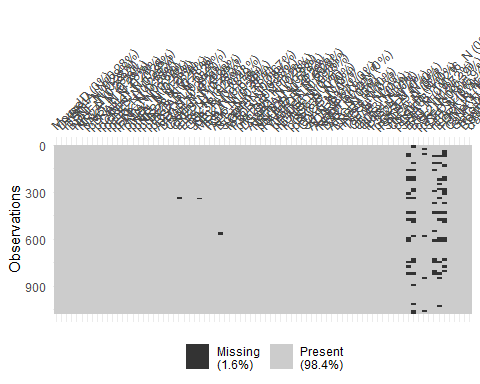
\includegraphics{512_project_files/figure-latex/unnamed-chunk-3-1.pdf}

As is observed in the plot of missing values, a few of the proteins
towards the right of the plot are missing quite a few observations, so
some data imputing must be done.

It would be useful to see the distribution of observations for the
different proteins.

\begin{Shaded}
\begin{Highlighting}[]
\CommentTok{\# boxplots of data}

\NormalTok{combined\_proteins}\OtherTok{\textless{}{-}}\FunctionTok{melt}\NormalTok{(}\AttributeTok{data=}\NormalTok{Data,}\AttributeTok{id.vars =} \FunctionTok{c}\NormalTok{(}\StringTok{"class"}\NormalTok{))}
\CommentTok{\# print("ggplot")}
\CommentTok{\# cat("\textbackslash{}n")}
\CommentTok{\# ggplot(data=combined\_proteins)+}
\CommentTok{\#   geom\_boxplot(mapping=aes(class,value)) \# box plot of all values by class}
\CommentTok{\# cat("\textbackslash{}n")}
\FunctionTok{print}\NormalTok{(}\StringTok{"base"}\NormalTok{)}
\end{Highlighting}
\end{Shaded}

\begin{verbatim}
## [1] "base"
\end{verbatim}

\begin{Shaded}
\begin{Highlighting}[]
\FunctionTok{cat}\NormalTok{(}\StringTok{"}\SpecialCharTok{\textbackslash{}n}\StringTok{"}\NormalTok{)}
\end{Highlighting}
\end{Shaded}

\begin{Shaded}
\begin{Highlighting}[]
\FunctionTok{boxplot}\NormalTok{(value}\SpecialCharTok{\textasciitilde{}}\NormalTok{class,}\AttributeTok{data=}\NormalTok{combined\_proteins,}\AttributeTok{xlab =} \StringTok{"class"}\NormalTok{,}\AttributeTok{ylab=}\StringTok{"protein levels"}\NormalTok{) }\CommentTok{\# boxplot of all values by class}
\FunctionTok{title}\NormalTok{(}\AttributeTok{main=}\StringTok{"Protein expression levels by class(all proteins combined)"}\NormalTok{)}
\end{Highlighting}
\end{Shaded}

\includegraphics{512_project_files/figure-latex/unnamed-chunk-5-1.pdf}

\begin{Shaded}
\begin{Highlighting}[]
\FunctionTok{cat}\NormalTok{(}\StringTok{"}\SpecialCharTok{\textbackslash{}n}\StringTok{"}\NormalTok{)}
\end{Highlighting}
\end{Shaded}

\begin{Shaded}
\begin{Highlighting}[]
\DocumentationTok{\#\#next boxplot of averages of protein values for each class }
\CommentTok{\# data\_combined\textless{}{-}matrix(,ncol=78,nrow=8)}
\CommentTok{\# for (i in 1:77)\{}
\CommentTok{\#   data\_combined[,i]\textless{}{-}mean(Data[,i]\textasciitilde{}Data$class)}
\CommentTok{\# \}}
\CommentTok{\# classes\textless{}{-}names(mean(Data[,1]\textasciitilde{}Data$class))}
\CommentTok{\# dim(data\_combined)}
\CommentTok{\# data\_combined[,78]\textless{}{-}classes}
\CommentTok{\# colnames(data\_combined)[colnames(data\_combined)=="V78"]\textless{}{-}"class"}
\end{Highlighting}
\end{Shaded}

\begin{Shaded}
\begin{Highlighting}[]
\CommentTok{\# data\_combined\textless{}{-}melt(data\_combined,id.vars=c("class"))}
\CommentTok{\# for (i in 1:624)\{}
\CommentTok{\#   id\textless{}{-}data\_combined[i,1]}
\CommentTok{\#   data\_combined[i,1]\textless{}{-}classes[as.numeric(id)]}
\CommentTok{\# \}}
\CommentTok{\# data\_combined\textless{}{-}subset(data\_combined,select = {-}Var2)}
\CommentTok{\# print("plots of all average expressions by protein")}
\CommentTok{\# cat("\textbackslash{}n")}
\CommentTok{\# print("base")}
\CommentTok{\# cat("\textbackslash{}n")}
\CommentTok{\# boxplot(as.numeric(data\_combined$value)\textasciitilde{}data\_combined$Var1,ylab = "protein expression",xlab="class")}
\CommentTok{\# title(main="Protein expression levels by class(combined class averages for each protein)")}
\CommentTok{\# cat("\textbackslash{}n")}
\CommentTok{\# print("ggplot")}
\CommentTok{\# cat("\textbackslash{}n")}
\CommentTok{\# ggplot(data\_combined)+}
\CommentTok{\#   geom\_boxplot(mapping=aes(Var1,as.numeric(value))) +}
\CommentTok{\#   xlab("class") +}
\CommentTok{\#   ylab("protein expression") +}
\CommentTok{\#   ggtitle("Protein expression levels by class(combined class averages for each protein")}
\end{Highlighting}
\end{Shaded}

\includegraphics{512_project_files/figure-latex/unnamed-chunk-7-1.pdf}

It looks like some proteins have quite a large difference in
measurements across classes. It would make sense to fit multiple mean
models to the different proteins to see if there is a difference.

\emph{\textbf{H\_null}: there are no differences in expression level
mean between classes.}

\[H_0: \mu_0=\mu_1 = \mu_2 = \mu_3 = \mu_4 = \mu_5 = \mu_6 = \mu_7 \]
\emph{\textbf{H\_alt}: there is at least one significant difference
among the groups.}

\[H_A: \mu_0 \neq \mu_1 \neq \mu_2 \neq \mu_3 \neq \mu_4 \neq \mu_5 \neq \mu_6 \neq \mu_7 \neq \mu_8\]

\textbf{Model fitting}

We fit a simple model to each protein :

\(\mu\)\{Protein\textbar c-CS-m,c-SC-m,c-CS-s,c-SC-s,t-CS-m,t-SC-m,t-CS-s,t-SC-s\}\(=\beta_0 +\beta_1I_{c-SC-m}+\beta_2I_{c-CS-s}+\beta_3I_{c-SC-s}+\beta_4I_{t-CS-m}+\beta_5I_{t-SC-m}+\beta_6I_{t-CS-s}+\beta_7I_{t-SC-s}\)

\texttt{lm\_herb1}: \[ I_{c-SC-m} = \begin{cases} 
          1 & \text{if class is c-SC-m} \\
          0 & \text{otherwise}
       \end{cases}
      \] \[ I_{c-CS-s} = \begin{cases} 
          1 & \text{if class is c-CS-s} \\
          0 & \text{otherwise}
       \end{cases}
      \] \[ I_{c-SC-s} = \begin{cases} 
          1 & \text{if class is c-SC-s} \\
          0 & \text{otherwise}
       \end{cases}
      \] \[ I_{t-CS-m} = \begin{cases} 
          1 & \text{if class is t-CS-m} \\
          0 & \text{otherwise}
       \end{cases}
      \] \[ I_{t-SC-m} = \begin{cases} 
          1 & \text{if class is t-SC-m} \\
          0 & \text{otherwise}
       \end{cases}
      \] \[ I_{t-SC-m} = \begin{cases} 
          1 & \text{if class is t-SC-m} \\
          0 & \text{otherwise}
       \end{cases}
      \] \[ I_{t-SC-s} = \begin{cases} 
          1 & \text{if class is t-SC-s} \\
          0 & \text{otherwise}
       \end{cases}
      \]

\begin{verbatim}
##            Protein Var_expl       p.value
## 1         DYRK1A_N     0.29  3.980441e-75
## 2          ITSN1_N     0.29  1.230006e-74
## 3           BDNF_N     0.11  8.725596e-24
## 4            NR1_N     0.09  1.357447e-19
## 5           NR2A_N     0.13  1.868668e-28
## 6           pAKT_N     0.19  1.779639e-45
## 7          pBRAF_N     0.16  1.320758e-36
## 8        pCAMKII_N     0.33  2.818994e-88
## 9          pCREB_N     0.11  7.944844e-24
## 10          pELK_N     0.11  9.005484e-23
## 11          pERK_N     0.36  4.569332e-99
## 12          pJNK_N     0.21  6.603188e-51
## 13          PKCA_N     0.16  5.708838e-38
## 14          pMEK_N     0.19  1.157002e-44
## 15          pNR1_N     0.11  5.342219e-25
## 16         pNR2A_N     0.31  5.188787e-82
## 17         pNR2B_N     0.11  1.000318e-22
## 18        pPKCAB_N     0.39 6.452687e-109
## 19          pRSK_N     0.08  3.286824e-16
## 20           AKT_N     0.23  3.370599e-57
## 21          BRAF_N     0.26  4.992471e-65
## 22        CAMKII_N     0.15  1.045206e-33
## 23          CREB_N     0.09  6.970974e-19
## 24           ELK_N     0.06  1.983440e-11
## 25           ERK_N     0.19  3.024075e-44
## 26         GSK3B_N     0.26  2.865826e-65
## 27           JNK_N     0.06  9.683309e-11
## 28           MEK_N     0.07  5.170426e-14
## 29          TRKA_N     0.08  2.068313e-15
## 30           RSK_N     0.05  5.885899e-10
## 31           APP_N     0.33  4.171656e-88
## 32      Bcatenin_N     0.08  1.451842e-15
## 33          SOD1_N     0.66 1.209388e-243
## 34          MTOR_N     0.27  5.161274e-70
## 35           P38_N     0.47 3.545236e-142
## 36         pMTOR_N     0.36  1.039129e-98
## 37         DSCR1_N     0.12  2.887391e-25
## 38         AMPKA_N     0.15  5.249088e-33
## 39          NR2B_N     0.27  2.816364e-68
## 40         pNUMB_N     0.30  4.061030e-80
## 41        RAPTOR_N     0.21  2.472756e-50
## 42         TIAM1_N     0.15  3.951100e-35
## 43        pP70S6_N     0.27  1.437178e-70
## 44          NUMB_N     0.17  6.765151e-40
## 45         P70S6_N     0.06  7.397068e-11
## 46        pGSK3B_N     0.36 7.114063e-100
## 47         pPKCG_N     0.25  1.082395e-62
## 48          CDK5_N     0.17  8.453641e-39
## 49            S6_N     0.39 1.250355e-110
## 50        ADARB1_N     0.13  2.549053e-30
## 51    AcetylH3K9_N     0.13  7.566911e-29
## 52          RRP1_N     0.03  1.475502e-05
## 53           BAX_N     0.07  6.381704e-14
## 54           ARC_N     0.48 1.728614e-145
## 55         ERBB4_N     0.19  7.883676e-46
## 56          nNOS_N     0.20  8.639413e-47
## 57           Tau_N     0.18  2.985743e-42
## 58          GFAP_N     0.14  3.946997e-32
## 59         GluR3_N     0.11  7.395391e-24
## 60         GluR4_N     0.02  2.040815e-03
## 61          IL1B_N     0.32  2.060474e-84
## 62         P3525_N     0.14  1.033929e-32
## 63        pCASP9_N     0.08  5.008883e-16
## 64         PSD95_N     0.18  1.390435e-41
## 65          SNCA_N     0.33  3.281180e-90
## 66     Ubiquitin_N     0.51 1.628986e-162
## 67 pGSK3B_Tyr216_N     0.07  9.536395e-14
## 68           SHH_N     0.08  1.039664e-17
## 69           BAD_N     0.10  2.102935e-20
## 70          BCL2_N     0.09  1.736128e-19
## 71           pS6_N     0.48 1.728614e-145
## 72         pCFOS_N     0.07  2.001019e-14
## 73           SYP_N     0.08  2.974103e-16
## 74       H3AcK18_N     0.17  1.058385e-38
## 75          EGR1_N     0.21  1.819861e-50
## 76        H3MeK4_N     0.19  7.181599e-44
## 77          CaNA_N     0.61 5.372624e-215
\end{verbatim}

\begin{Shaded}
\begin{Highlighting}[]
\NormalTok{AOV\_df}\SpecialCharTok{$}\NormalTok{reject\_null }\OtherTok{\textless{}{-}}\NormalTok{ AOV\_df}\SpecialCharTok{$}\NormalTok{p.value }\SpecialCharTok{\textless{}}\NormalTok{ alpha}
\NormalTok{alpha\_adj }\OtherTok{\textless{}{-}}\NormalTok{ alpha }\SpecialCharTok{/} \FunctionTok{length}\NormalTok{(}\FunctionTok{unique}\NormalTok{(Data}\SpecialCharTok{$}\NormalTok{class))}\SpecialCharTok{*}\NormalTok{(}\FunctionTok{length}\NormalTok{(}\FunctionTok{unique}\NormalTok{(Data}\SpecialCharTok{$}\NormalTok{class))}\SpecialCharTok{{-}}\DecValTok{1}\NormalTok{)}\SpecialCharTok{/}\DecValTok{2}
\end{Highlighting}
\end{Shaded}


\end{document}
